\documentclass[12pt, a4paper, twoside]{article}
\usepackage[margin=1in, headheight=0.3in, headsep=0.2in]{geometry}
\textwidth 16.5 cm \textheight 24cm
\oddsidemargin -2mm

% Packages
\usepackage{amsmath, listings, xcolor, tcolorbox, microtype, fancyhdr, hyperref, tikz}
\usetikzlibrary{decorations.pathreplacing}

% Configure text justification
\raggedbottom
\renewcommand{\textfraction}{0.05}
\renewcommand{\floatpagefraction}{0.85}
\renewcommand{\topfraction}{0.9}

% Configure the header
\setlength{\headheight}{14.49998pt}
\pagestyle{fancy}
\fancyhf{} 
\fancyhead[L]{\leftmark}
\fancyhead[R]{\thepage}
\renewcommand{\footrulewidth}{0pt}
\renewcommand{\sectionmark}[1]{\markboth{\thesection.~#1}{}}
\renewcommand{\subsectionmark}[1]{}

% Configure the links to look professional
\hypersetup{
    colorlinks=true,      % false: boxed links; true: colored links
    linkcolor=navyblue,   % Color of internal links (TOC, sections)
    citecolor=navyblue,   % Color of citations
    urlcolor=navyblue,    % Color of external URLs
    pdftitle={Numerical Solutions using WKB},  % Metadata for the PDF
    pdfauthor={Mohak Das}                      % Metadata for the PDF
}

% Define custom colors for code
\definecolor{codegreen}{rgb}{0,0.6,0}
\definecolor{codegray}{rgb}{0.5,0.5,0.5}
\definecolor{codepurple}{rgb}{0.58,0,0.82}
\definecolor{backcolour}{rgb}{0.95,0.95,0.92}
\definecolor{navyblue}{RGB}{0, 51, 102} % A professional deep blue

% Configure the Fortran style
\lstdefinestyle{codestyle}{
    backgroundcolor=\color{backcolour},   
    commentstyle=\color{codegreen},
    keywordstyle=\color{magenta},
    numberstyle=\tiny\color{codegray},
    stringstyle=\color{codepurple},
    basicstyle=\ttfamily\footnotesize, % Typewriter font, small size
    breakatwhitespace=false,         
    breaklines=true,                 % Break long lines automatically
    captionpos=b,                    % Caption at bottom
    keepspaces=true,                 
    numbers=left,                    % Line numbers on the left
    numbersep=5pt,                  
    showspaces=false,                
    showstringspaces=false,
    showtabs=false,                  
    tabsize=4,
    language=Fortran                 % Set language to Fortran
}

% Define a style for raw text output
\lstdefinestyle{outputstyle}{
    backgroundcolor=\color{white},   
    basicstyle=\ttfamily\small,      % Monospaced font
    breaklines=true,                 % Wrap long lines
    frame=single,                    % Add a black frame around the output
    numbers=none,                    % No line numbers
    captionpos=b,
    keepspaces=true
}

\begin{document}

    \begin{titlepage}
        \centering

        \vspace*{\fill}
        \Huge \textsc{\textcolor{navyblue}{Jadavpur University}}\\
        \LARGE \textsc{Department of Physics}\\[1cm]

        \textcolor{navyblue}{\rule{\linewidth}{0.8mm}} \\[0.4cm] 
        \Huge \textbf{\textcolor{navyblue}{Numerical Solutions using the \\ WKB Approximation}} \\[0.2cm]
        \textcolor{navyblue}{\rule{\linewidth}{0.8mm}} \\[1.5cm] 

        \large \textit{The Quantization Condition}\\[0.5cm]

        \begin{tcolorbox}[colback=navyblue!5!white, colframe=navyblue, width=0.8\textwidth, boxrule=0.5mm, arc=2mm, auto outer arc]
            \centering \Large
            $$ \int_{x_L}^{x_R} \sqrt{2m(E - V(x))} \, dx = \left(n + \alpha\right) \pi \hbar $$
        \end{tcolorbox}

        \vspace{1.5cm}

        \noindent
        \begin{minipage}{0.4\textwidth}
            \begin{flushleft} \Large
                \textbf{Submitted by:}\\
                \textcolor{navyblue}{Mohak Das}\\
            \end{flushleft}
        \end{minipage}
        \begin{minipage}{0.4\textwidth}
            \begin{flushright} \Large
                \textbf{Supervisor:} \\
                Dr. Asim Kumar Ghosh\\
                \vspace{0.6cm}
            \end{flushright}
        \end{minipage}
        \vspace{1cm}

        \textbf{Class:} PG-I\\
        \textbf{Class Roll No:} 002520702028\\
        \textbf{Exam Roll No:} PPHD0261034
        \vspace{1.5cm}

        \textsc{Computational Physics Lab}

        \vspace*{\fill}


    \end{titlepage}
    \thispagestyle{empty}

    \begin{abstract}
        This report presents the numerical application of the semiclassical Wentzel-Kramers-Brillouin (WKB) approximation to solve the time-independent Schrödinger equation for various one-dimensional potentials. A generalized Fortran 90 solver was developed using the Bohr-Sommerfeld quantization condition and the Bisection root-finding method. The solver was tested against eleven distinct potentials, including harmonic, infinite well, and anharmonic systems. The numerical results show excellent agreement with exact analytical values for the Harmonic Oscillator ($>99.99\%$ accuracy) and the Infinite Square Well, validating the solver's robustness. For anharmonic potentials where exact solutions are not available, the results exhibit the expected physical scaling behavior.
    \end{abstract}
    
    \thispagestyle{empty}
    \newpage

  	\tableofcontents
	\thispagestyle{empty}
	
	\clearpage
	\pagenumbering{arabic}

    \section{Introduction}

        \subsection{Main Idea}
        The Wentzel–Kramers–Brillouin (WKB) approximation is a semiclassical method used in quantum mechanics to solve the time-independent Schrödinger equation. It is particularly useful for systems where the potential energy $V(x)$ varies slowly compared to the de Broglie wavelength of the particle. While exact analytical solutions are rare for arbitrary potentials, the WKB method provides a powerful tool to approximate the wavefunction and, crucially, to calculate accurate energy eigenvalues for bound states without solving the full differential equation.

        \subsection{The Approximation}
        The method starts by assuming the wavefunction $\psi(x)$ can be written in the form of a plane wave with a slowly varying amplitude and phase. The ansatz is: 
        $$\boxed{\psi(x) \approx {\frac{C}{\sqrt{p(x)} } e^{ \pm \frac{i}{\hbar} \int p(x) \, dx} }}$$

        where $p(x) = \sqrt{2m(E-V(x))}$ is the classical momentum of the particle. This approximation holds true in regions where the potential $V(x)$ changes slowly enough that the change in the particle's momentum over one wavelength is small.

        \subsection{The Quantization Condition}
        For bound states, the particle is confined between turning points (where $E = V(x)$). By matching the oscillatory solutions inside the potential well with the exponentially decaying solutions in the classically forbidden regions (using Airy functions near the turning points), we derive a constraint on the action integral. The general Bohr-Sommerfeld quantization condition is:
        $$ \boxed{{\int_{x_1}^{x_2} p(x) \, dx} = {\int_{x_1}^{x_2} \sqrt{2m(E-V(x))} \, dx} = {\left(n+\alpha\right) \pi \hbar}} $$

        where $x_1$ and $x_2$ are the boundaries of the motion, $n$ is an integer quantum number, and $\alpha$ is a phase constant determined by the boundary conditions (e.g., rigid walls vs. soft potential slopes).

        \begin{figure}[b]
        \centering
        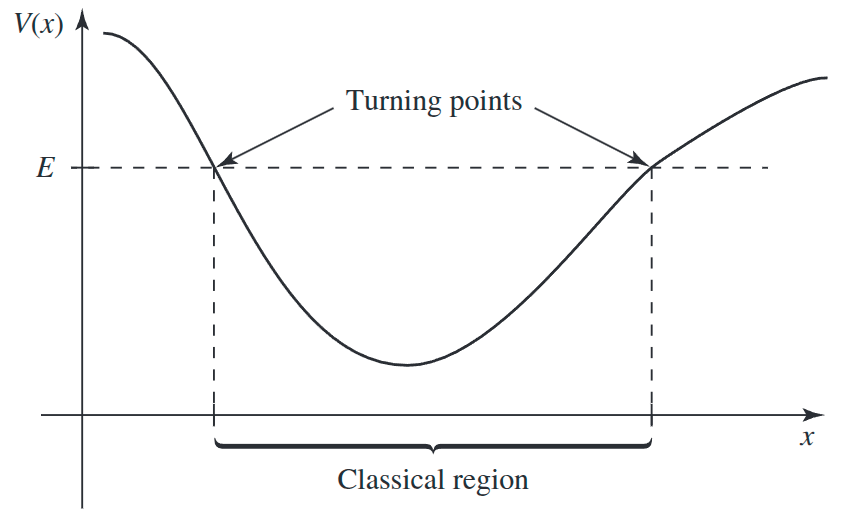
\includegraphics[width=0.32183\textwidth]{WKB_Diagram.png}
        \caption{Schematic of the WKB approximation. The particle is confined between classical turning points $x_L$ and $x_R$, where the energy $E$ intersects the potential $V(x)$.}
        \label{fig:wkb_scheme}
        \end{figure}

    \section{Numerical Implementation}

        \subsection{Global Constants and Precision}
        To ensure numerical stability and physical consistency across all problems, a shared module \texttt{constants\_mod} is used. This module defines the double-precision floating-point kind (\texttt{real64}) and sets the atomic units ($\hbar = 1, m = 1$).

        \lstinputlisting[caption={Global Constants Module}, style= codestyle, label={lst:const}]{src/shared/constants_mod.f90}

        \subsection{The General WKB Solver}
        The core logic is encapsulated in the \texttt{wkb\_toolbox} module.
        
        \subsubsection*{The WKB Solver}
        The computational approach treats the quantization condition as a root-finding problem. For a given quantum number $n$ and phase factor $\alpha$, we seek the energy $E$ that satisfies:
        $$ f(E) = \int_{x_L}^{x_R} \sqrt{2m(E - V(x))} \, dx - (n + \alpha)\pi \hbar = 0 $$
        The solver employs the \textbf{Bisection Method}, a robust root-finding algorithm. It iteratively narrows the energy bracket $[E_{min}, E_{max}]$ by evaluating the action integral at the midpoint and checking the sign of the residual. This method ensures convergence to the global solution for the monotonic action function.
        
        \subsubsection*{Choice of Integration Scheme: Trapezoidal Rule}
        The action integral is computed using the \textbf{Composite Trapezoidal Rule}. This method was selected specifically for its stability in the context of WKB integrals:
        \begin{itemize}
            \item \textbf{Boundary Behavior:} The integrand $p(x) = \sqrt{2m(E-V(x))}$ vanishes identically at the classical turning points ($x_L, x_R$). The Trapezoidal rule incorporates these zero-valued endpoints naturally without requiring special handling.
            \item \textbf{Singularity Avoidance:} The derivative of the momentum function becomes singular at the turning points (since $\frac{d}{dx}\sqrt{x} \to \infty$ as $x \to 0$). Higher-order methods like Simpson's rule or Gaussian quadrature can be sensitive to such non-smooth behavior at the boundaries. The Trapezoidal rule, which relies solely on function evaluations rather than derivatives, remains numerically stable and sufficiently accurate for this class of integrals.
        \end{itemize}
        \lstinputlisting[caption={WKB Toolbox Implementation}, style= codestyle, label={lst:solver}]{src/shared/wkb_toolbox.f90}
    
    \section{Solution to the Assignment Problems}
        \subsection{Problem 1: One-dimensional Half-Harmonic Potential}
        \begin{itemize}
            \item {\bf Potential: } $V(x) = \frac{1}{2} m \omega^2 x^2$ for $x \geq 0,~ \infty $ otherwise.
            \item {\bf Quantization Condition Used: } One Rigid Wall, One Soft Turning Point. $${\int_{0}^{x_R} \sqrt{2m(E-V(x))} \, dx} = {\left(n - \frac{1}{4}\right) \pi \hbar} ~~ (n = 1, 2, \cdots)$$
            \item {\bf Reason: } The potential has a "hard wall" at $x=0$ (infinite potential), forcing the wavefunction to vanish ($\psi(0)=0$). The other boundary $x_R$ is a "soft" turning point where the potential slopes gently. The phase shift contribution is $0$ from the hard wall and $-\pi/4$ from the soft turning point, leading to the $(n - 1/4)$ factor.
            \item {\bf Turning Point Calculation: } At the turning points, kinetic energy $E$ is equal to potential energy $V(x)$. $$E = V(x)$$ \begin{alignat*}{2}
                &\implies ~ E = \frac{1}{2} m \omega^2 x^2 \\
                &\implies ~ x^2 = \frac{2E}{m \omega^2} \\
                &\implies ~ x = \pm \sqrt{\frac{2E}{m \omega^2}}
            \end{alignat*} 
            using $m = 1$ and $\omega = 1$, we get the right turning point $ \boxed{x_R = \sqrt{2E}}$. Since this is a Half-Harmonic potential, the left turning point $\boxed{x_L = 0}$.
            
            \item {\bf Code: } \lstinputlisting[style= codestyle]{src/problems/prob01_half_harmonic.f90}
            \item {\bf Output: } \lstinputlisting[style= outputstyle]{output/prob01_output.txt}
        \end{itemize}
        
        \subsection{Problem 2: One-dimensional Harmonic Potential}
        \begin{itemize}
            \item {\bf Potential: } $V(x) = \frac{1}{2} m \omega^2 x^2$.
            \item {\bf Quantization Condition Used: } Two Soft Turning Points. $${\int_{x_L}^{x_R} \sqrt{2m(E-V(x))} \, dx} = {\left(n + \frac{1}{2}\right) \pi \hbar} ~~ (n = 0, 1, \cdots)$$
            \item {\bf Reason: }  The particle is confined by the potential on both sides without any hard walls. Both turning points $x_L$ and $x_R$ are "soft" (linear turning points), each contributing a phase shift of $-\pi/4$. The total phase loss is $\pi/2$, resulting in the standard $(n + 1/2)$ term.
            \item {\bf Turning Point Calculation: } At the turning points, kinetic energy $E$ is equal to potential energy $V(x)$. $$E = V(x)$$ \begin{alignat*}{2}
                &\implies ~ E = \frac{1}{2} m \omega^2 x^2 \\
                &\implies ~ x^2 = \frac{2E}{m \omega^2} \\
                &\implies ~ x = \pm \sqrt{\frac{2E}{m \omega^2}}
            \end{alignat*}
            using $m = 1$ and $\omega = 1$, we get the right turning point $ \boxed{x_R = \sqrt{2E}}$ and the left turning point $\boxed{x_L = -\sqrt{2E}}$.
            \item {\bf Code: } \lstinputlisting[style= codestyle]{src/problems/prob02_1D_harmonic.f90}
            \item {\bf Output: } \lstinputlisting[style= outputstyle]{output/prob02_output.txt}
        \end{itemize}
        
        \subsection{Problem 3: One-dimensional Infinite Square Well Potential}
        \begin{itemize}
            \item {\bf Potential: } $V(x) = 0$ for $-L \leq x \leq L, ~\infty$ otherwise.
            \item {\bf Quantization Condition Used: } Two Rigid Walls. $${\int_{-L}^{L} \sqrt{2mE} \, dx} = {n \pi \hbar} ~~ (n = 1, 2, \cdots)$$
            \item {\bf Reason: }  The particle is confined strictly between $x=-L$ and $x=L$ by infinite potential barriers. The wavefunction must be exactly zero at both boundaries. There are no "soft" turning points region to generate the $\pi/4$ phase shifts, so the phase factor $\alpha$ is zero.
            \item {\bf Code: } \lstinputlisting[style= codestyle]{src/problems/prob03_infinite_square_well.f90}
            \item {\bf Output: } \lstinputlisting[style= outputstyle]{output/prob03_output.txt}
        \end{itemize}
        
        \subsection{Problem 4: Infinite Potential Well with Slanted Base}
        \begin{itemize}
            \item {\bf Potential: } $V(x) = \frac{V_0}{L} x$ for $0 \leq x \leq L, ~\infty$ otherwise.
            \item {\bf Quantization Condition Used: } One Rigid Wall, One Soft Turning Point. $${\int_{0}^{x_R} \sqrt{2m(E-V(x))} \, dx} = {\left(n - \frac{1}{4}\right) \pi \hbar} ~~ (n = 1, 2, \cdots)$$
            \item {\bf Reason: }  For the low-lying energy states calculated ($E < V_0$), the particle turns back at a point $x_R < L$ where $E=V(x)$. Thus, the system effectively has one hard wall at $x=0$ and one soft classical turning point at $x_R$.
            \item {\bf Turning Point Calculation: } At the turning points, kinetic energy $E$ is equal to potential energy $V(x)$. $$E = V(x)$$ \begin{alignat*}{2}
                &\implies ~ E = \frac{V_0}{L} x \\
                &\implies ~ x = \frac{L}{V_0} E
            \end{alignat*}
            Thus, the right turning point $ \boxed{x_R = \frac{L}{V_0} E}$.
            \item {\bf Code: } \lstinputlisting[style= codestyle]{src/problems/prob04_infinite_potential_well_slanted_base.f90}
            \item {\bf Output: } \lstinputlisting[style= outputstyle]{output/prob04_output.txt}
        \end{itemize}
        
        \subsection{Problem 5: Infinite Potential Well with Parabolic Base}
        \begin{itemize}
            \item {\bf Potential: } $V(x) = \frac{V_0}{L^2} x^2$ for $0 \leq x \leq L, ~\infty$ otherwise.
            \item {\bf Quantization Condition Used: } One Rigid Wall, One Soft Turning Point. $${\int_{0}^{x_R} \sqrt{2m(E-V(x))} \, dx} = {\left(n - \frac{1}{4}\right) \pi \hbar} ~~ (n = 1, 2, \cdots)$$
            \item {\bf Reason: }  Similar to the slanted well, for energies $E < V_0$, the particle is confined by the hard wall at $x=0$ and a soft turning point $x_R$ formed by the parabolic potential.
            \item {\bf Turning Point Calculation: } At the turning points, kinetic energy $E$ is equal to potential energy $V(x)$. $$E = V(x)$$ \begin{alignat*}{2}
                &\implies ~ E = \frac{V_0}{L^2} x^2 \\
                &\implies ~ x^2 = \frac{L^2}{V_0} E
                &\implies ~ x = \pm \sqrt{\frac{L^2}{V_0}E}
            \end{alignat*}
            Thus, the right turning point $ \boxed{x_R = L \sqrt{\frac{E}{V_0}}}$.
            \item {\bf Code: } \lstinputlisting[style= codestyle]{src/problems/prob05_parabolic_base.f90}
            \item {\bf Output: } \lstinputlisting[style= outputstyle]{output/prob05_output.txt}
        \end{itemize}
        
        \subsection{Problem 6: \texorpdfstring{$V(x) = |x|$}{V(x) = |x|}}
        \begin{itemize}
            \item {\bf Potential: } $V(x) = |x|$.
            \item {\bf Quantization Condition Used: } Two Soft Turning Points. $${\int_{x_L}^{x_R} \sqrt{2m(E - |x|)} \, dx} = {\left(n + \frac{1}{2}\right) \pi \hbar} ~~ (n = 0, 1, \cdots)$$
            \item {\bf Reason: }  The potential is continuous and confining on both sides ($x \to \pm \infty$). There are no infinite walls, so the standard WKB rule for two soft turning points applies.
            \item {\bf Turning Point Calculation: } At the turning points, kinetic energy $E$ is equal to potential energy $V(x)$. $$E = V(x)$$ \begin{alignat*}{2}
                &\implies ~ E = |x|
            \end{alignat*}
            $E = x $ for $x \geq 0$ and $E = -x$ for $x < 0$.
            Thus, the right turning point $ \boxed{x_R = E}$ and the left turning point $\boxed{x_L = -E}$.
            \item {\bf Code: } \lstinputlisting[style= codestyle]{src/problems/prob06_modx.f90}
            \item {\bf Output: } \lstinputlisting[style= outputstyle]{output/prob06_output.txt}
        \end{itemize}

        \subsection{Problem 7: \texorpdfstring{$V(x) = |x^3|$}{V(x) = |x\^{}3|}}
        \begin{itemize}
            \item {\bf Potential: } $V(x) = |x^3|$.
            \item {\bf Quantization Condition Used: } Two Soft Turning Points. $${\int_{x_L}^{x_R} \sqrt{2m(E - |x^3|)} \, dx} = {\left(n + \frac{1}{2}\right) \pi \hbar} ~~ (n = 0, 1, \cdots)$$
            \item {\bf Reason: }  The potential is continuous and confining on both sides ($x \to \pm \infty$). There are no infinite walls, so the standard WKB rule for two soft turning points applies.
            \item {\bf Turning Point Calculation: } At the turning points, kinetic energy $E$ is equal to potential energy $V(x)$. $$E = V(x)$$ \begin{alignat*}{2}
                &\implies ~ E = |x^3|
            \end{alignat*}
            $E = x^3 $ for $x \geq 0$ and $E = -x^3$ for $x < 0$.
            Thus, the right turning point $ \boxed{x_R = \sqrt[3]{E}}$ and the left turning point $\boxed{x_L = -\sqrt[3]{E}}$.
            \item {\bf Code: } \lstinputlisting[style= codestyle]{src/problems/prob07_modx_cube.f90}
            \item {\bf Output: } \lstinputlisting[style= outputstyle]{output/prob07_output.txt}
        \end{itemize}
        
        \subsection{Problem 8: \texorpdfstring{$V(x) = x^4$}{V(x) = x\^{}4}}
        \begin{itemize}
            \item {\bf Potential: } $V(x) = x^4$.
            \item {\bf Quantization Condition Used: } Two Soft Turning Points. $${\int_{x_L}^{x_R} \sqrt{2m(E - x^4)} \, dx} = {\left(n + \frac{1}{2}\right) \pi \hbar} ~~ (n = 0, 1, \cdots)$$
            \item {\bf Reason: }  The potential is continuous and confining on both sides ($x \to \pm \infty$). There are no infinite walls, so the standard WKB rule for two soft turning points applies.
            \item {\bf Turning Point Calculation: } At the turning points, kinetic energy $E$ is equal to potential energy $V(x)$. $$E = V(x)$$ \begin{alignat*}{2}
                &\implies ~ E = x^4
            \end{alignat*}
            Thus, the right turning point $ \boxed{x_R = \sqrt[4]{E}}$ and the left turning point $\boxed{x_L = -\sqrt[4]{E}}$.
            \item {\bf Code: } \lstinputlisting[style= codestyle]{src/problems/prob08_quartic_potential.f90}
            \item {\bf Output: } \lstinputlisting[style= outputstyle]{output/prob08_output.txt}
        \end{itemize}
        
        \subsection{Problem 9: \texorpdfstring{$V(x) = x^2 + x^4$}{V(x) = x\^{}2 + x\^{}4}}
        \begin{itemize}
            \item {\bf Potential: } $V(x) = x^2 + x^4$.
            \item {\bf Quantization Condition Used: } Two Soft Turning Points. $${\int_{x_L}^{x_R} \sqrt{2m(E - (x^2 + x^4))} \, dx} = {\left(n + \frac{1}{2}\right) \pi \hbar} ~~ (n = 0, 1, \cdots)$$
            \item {\bf Reason: }  The potential is continuous and confining on both sides ($x \to \pm \infty$). There are no infinite walls, so the standard WKB rule for two soft turning points applies.
            \item {\bf Turning Point Calculation: } The potential is given by:
            $$ V(x) = x^2 + x^4 $$
            The classical turning points $x_{tp}$ occur where the total energy equals the potential energy:
            $$ E = V(x_{tp}) \implies x^4 + x^2 - E = 0 $$
            This is a quadratic equation in terms of $x^2$. We can solve for $x^2$ using the quadratic formula:
            $$ x^2 = \frac{-1 \pm \sqrt{1 - 4(1)(-E)}}{2} = \frac{-1 \pm \sqrt{1 + 4E}}{2} $$
            Since $x^2$ must be non-negative (real coordinate space), we discard the negative root. Thus:
            $$ x^2 = \frac{\sqrt{1 + 4E} - 1}{2} $$
            Taking the square root, we obtain the symmetric turning points $\pm x_R$:
            $$ \boxed{x_R = \sqrt{\frac{\sqrt{1 + 4E} - 1}{2}}} $$
            The integration is performed between $x_L = -x_R$ and $x_R$.
            \item {\bf Code: } \lstinputlisting[style= codestyle]{src/problems/prob09_quadratic_quartic.f90}
            \item {\bf Output: } \lstinputlisting[style= outputstyle]{output/prob09_output.txt}
        \end{itemize}

        \subsection{Problem 10: One-dimensional Half-Cubic Potential}
        \begin{itemize}
            \item {\bf Potential: } $V(x) = x^3$ for $x \geq 0$, $\infty$ otherwise.
            \item {\bf Quantization Condition Used: } One Rigid Wall, One Soft Turning Point. $${\int_{0}^{x_R} \sqrt{2m(E - x^3)} \, dx} = {\left(n - \frac{1}{4}\right) \pi \hbar} ~~ (n = 1, 2, \cdots)$$
            \item {\bf Reason: }  The potential has an infinite barrier (hard wall) at $x=0$ and a standard soft turning point at $x_R$ determined by the cubic term.
            \item {\bf Turning Point Calculation: } At the turning points, kinetic energy $E$ is equal to potential energy $V(x)$. $$E = V(x)$$ \begin{alignat*}{2}
                &\implies ~ E = x^3
            \end{alignat*}
            The right turning point $ \boxed{x_R = \sqrt[3]{E}}$. Since this is a Half-Cubic potential, the left turning point $\boxed{x_L = 0}$.
            \item {\bf Code: } \lstinputlisting[style= codestyle]{src/problems/prob10_half_cubic.f90}
            \item {\bf Output: } \lstinputlisting[style= outputstyle]{output/prob10_output.txt}
        \end{itemize}

        \subsection{Problem 11: One-dimensional Half-Quartic Potential}
        \begin{itemize}
            \item {\bf Potential: } $V(x) = x^4$ for $x \geq 0$, $\infty$ otherwise.
            \item {\bf Quantization Condition Used: } One Rigid Wall, One Soft Turning Point. $${\int_{0}^{x_R} \sqrt{2m(E - x^4)} \, dx} = {\left(n - \frac{1}{4}\right) \pi \hbar} ~~ (n = 1, 2, \cdots)$$
            \item {\bf Reason: }  The potential has an infinite barrier (hard wall) at $x=0$ and a standard soft turning point at $x_R$ determined by the quartic term.
            \item {\bf Turning Point Calculation: } At the turning points, kinetic energy $E$ is equal to potential energy $V(x)$. $$E = V(x)$$ \begin{alignat*}{2}
                &\implies ~ E = x^4
            \end{alignat*}
            The right turning point $ \boxed{x_R = \sqrt[4]{E}}$. Since this is a Half-Cubic potential, the left turning point $\boxed{x_L = 0}$.
            \item {\bf Code: } \lstinputlisting[style= codestyle]{src/problems/prob11_half_quartic.f90}
            \item {\bf Output: } \lstinputlisting[style= outputstyle]{output/prob11_output.txt}
        \end{itemize}

    \section{Remarks}
    \begin{enumerate}
        \item WKB is exact for harmonic oscillator and infinite square well.
        \item For linear turning points (triangular well), results differ slightly from exact Airy-function values due to lack of explicit Airy matching.
        \item Accuracy improves for higher quantum numbers, as expected.
    \end{enumerate}
\end{document}